

 \subsection[Other priors]{Priors beyond the DP}
 
 \begin{frame}{Need for a power-law for $K_n$}
 	\citet{newman2005power,clauset2009power} show that ``\textit{Power-law distributions occur in many situations of scientific interest and have
significant consequences for our understanding of natural and man-made phenomena}''.
		\visible<2->{
		\begin{center}
			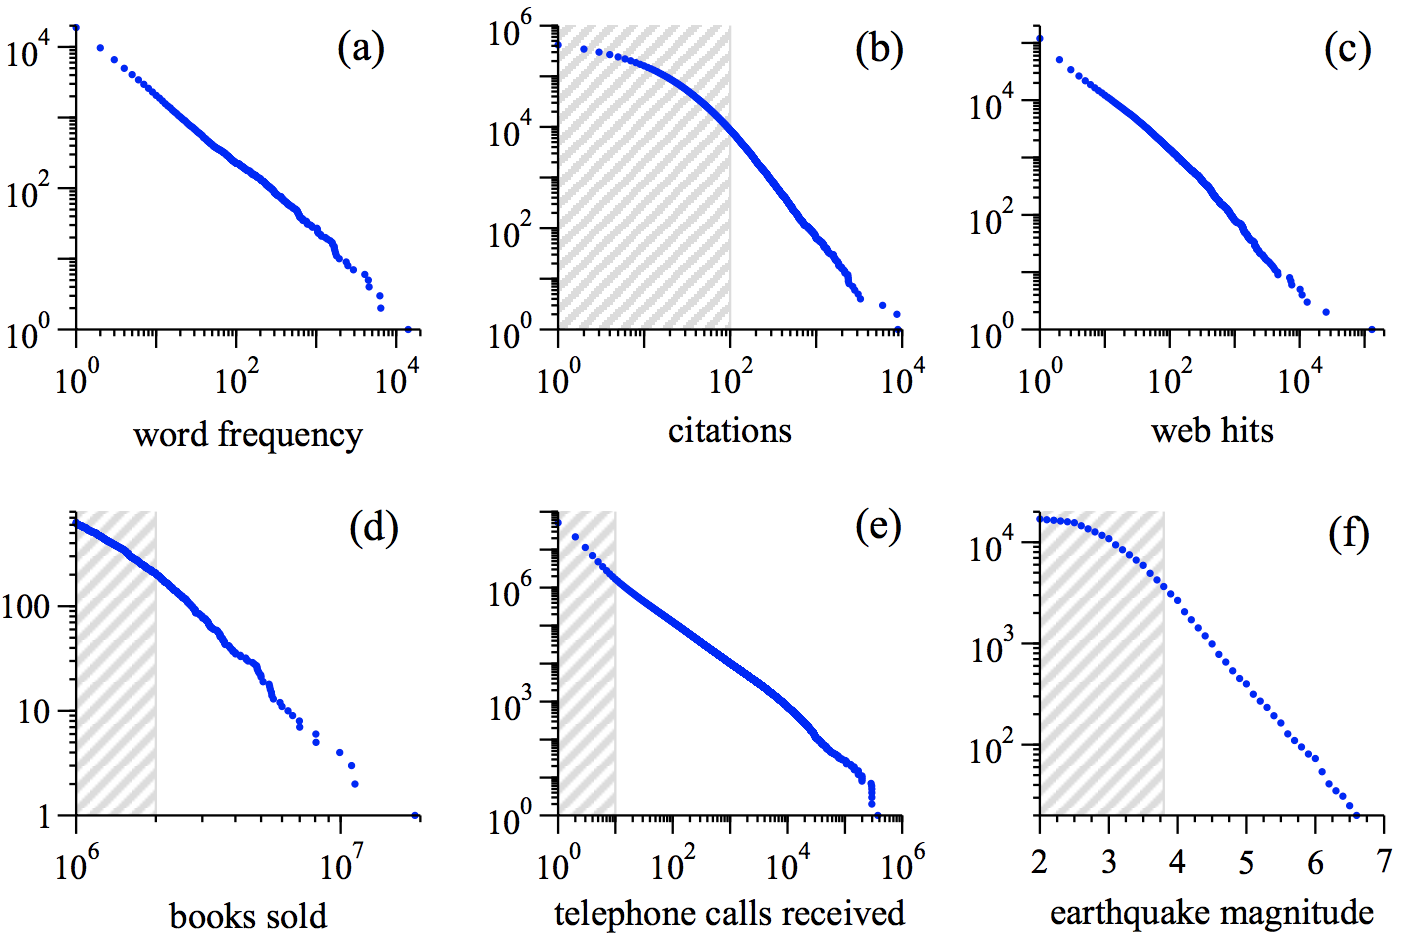
\includegraphics[width=.7\textwidth]{figures_julyan/beyond_DP/power_laws_newman}
		\end{center}
		\hfill\textcolor{gray}{[Image from \citet{newman2005power}]}\\
		}\pause
		Hence the need to depart from $K_n\sim \alpha \log n$ induced by a Dirichlet process.
 \end{frame}

 
\begin{frame}{Chinese restaurant process}
Consider discrete data $X_1,\ldots X_n\vert P\simiid P$, and $ P \sim \mathcal{Q}$

Features $k_n\leq n$ unique values $X_1^*,\ldots,X_{k_n}^*$ with resp. frequencies $n_1,\ldots,n_{k_n}$\medskip 


{Discrete random probability measures} are characterized by  \alert{predictive distr.}
\medskip

\only<1>{\alert{Dirichlet process} by \citet{ferguson1973bayesian}: $P\sim DP(\alpha, G_0)$

$$\P[X_{n+1}\in \cdot\, \vert\, X_1,\ldots X_{n}]=\frac{\alpha}{\alpha+n}G_{0}(.)+\frac{1}{\alpha+n}\sum_{j=1}^{{k_n}}n_j\delta_{X_{j}^*}(.)$$

\begin{center}
Log rate for number of clusters \alert{$k_n \asymp \alpha \log n$}
\end{center}

\medskip

\textcolor{gray}{
Product form exchangeable partition probability function  
$$p(n_1,\ldots,n_{k_n})=\alpha^{k_n}\frac{\Gamma(\alpha)}{\Gamma(\alpha+k_n)}\prod_{j=1}^{k_n}(n_j-1)!$$}
}


\only<2>{\alert{Pitman--Yor process} by \citet{pitman1997two}: $P\sim PY(\alert{\sigma},\alpha, G_0),\,\sigma\in(0,1)$

$$\P[X_{n+1}\in \cdot\, \vert\, X_1,\ldots X_{n}]=\frac{\alpha+\alert{\sigma k_n}}{\alpha+n}G_{0}(.)+\frac{1}{\alpha+n}\sum_{j=1}^{{k_n}}(n_j-\alert{\sigma})\delta_{X_{j}^*}(.)$$

\begin{center}
Power law rate for number of clusters \alert{$k_n \asymp S n^\sigma$}
\end{center}

\medskip

\textcolor{gray}{
Product form exchangeable partition probability function  
$$p(n_1,\ldots,n_{k_n})=\frac{\prod_{i=1}^{k_n-1}(\alpha+i\sigma)}{(\alpha+1)_{(n-1)}}\prod_{j=1}^{k_n}(1-\sigma)_{(n_j-1)}$$}
}


\only<3>{\alert{Gibbs-type processes} by \citet{pitman2003poisson}: $P\sim Gibbs(\alert{\sigma},(V_{n,k})_{n,k}, G_0),\,\sigma<1$

$$\P[X_{n+1}\in \cdot\, \vert\, X_1,\ldots X_{n}]=\alert{\frac{V_{n+1,{k_n}+1}}{V_{n,{k_n}}}}G_{0}(.)+\alert{\frac{V_{n+1,{k_n}}}{V_{n,{k_n}}}}\sum_{j=1}^{{k_n}}(n_j-\alert{\sigma})\delta_{X_{j}^*}(.)$$

\begin{center}
Rate for number of clusters 
$\alert{k_n \asymp }
\left\{
\begin{array}{l}
\alert{K} \text{ random variable a.s. finite if }\sigma<0\\
\alert{\alpha \log n}  \text{  if }\sigma=0\\
\alert{S n^\sigma} \text{ if }\sigma\in(0,1), (S \text{ random variable)}.
\end{array}
\right.
$
\end{center}
\medskip

\textcolor{gray}{
Product form exchangeable partition probability function  
$$p(n_1,\ldots,n_{k_n})=V_{n,{k_n}}\prod_{j=1}^{k_n}(1-\sigma)_{(n_j-1)}$$}
}
\end{frame}



\begin{frame}{Beyond the DP from predictive function viewpoint} 
%According to the de Finetti representation theorem, $(X_{i})_{i\geq1}$ is an exchangeable sequence. The distribution of such a sequence, and hence $\mathscr{Q}$, is 
%characterized by conditional probability of discovering a new species at $(n+1)$-th step, i.e.
%\vspace{0.1cm}
%\begin{equation}\label{eq:newspecies} \tag{$\ast$}
%\P[X_{n+1}\hbox{ is ``new''} \: |\: \boldsymbol{X}_{n}].
%\end{equation}

A discrete random probability measure $P$ can be classified in 3 main categories according to $\P[X_{n+1}\hbox{ is ``new''} \: |\: \boldsymbol{X}_{n}]$
    \begin{itemize}
    \smallskip
    \item<2->[1)] $\P[X_{n+1}\hbox{ is ``new''} \: |\: \boldsymbol{X}_{n}]=\alert{f(n, \hbox{model parameters})}$

     $ \hspace{1.2cm} \Longleftrightarrow \ $ depends on $n$ but not on $k_{n}$ and $(n_{1},\ldots,n_{k_{n}})$

     $ \hspace{1.2cm} \Longleftrightarrow \ $ Dirichlet process \citep{ferguson1973bayesian};\\[4pt]
     
    \smallskip

    \item<3->[2)] $\P[X_{n+1}\hbox{ is ``new''} \: |\: \boldsymbol{X}_{n}]=\textcolor{red2}{f(n, k_{n}, \hbox{model parameters})}$

    $ \hspace{1.2cm} \Longleftrightarrow \ $ depends on $n$ and $k_{n}$  but not on $(n_{1},\ldots,n_{k_{n}})$

    $ \hspace{1.2cm} \Longleftrightarrow \ $\textcolor{red2}{Gibbs-type prior} \citep{pitman2003poisson};\\[4pt]

\smallskip

    \item<4->[3)] $\P[X_{n+1}\hbox{ is ``new''} \: |\: \boldsymbol{X}_{n}]=\alert{f(n, k_{n}, (n_{1},\ldots,n_{k_{n}}), \hbox{model parameters})}$

    $ \hspace{1.2cm} \Longleftrightarrow \ $ depends on  $n$, $k_{n}$ and $(n_{1},\ldots,n_{k_{n}})$
    
    $ \hspace{1.2cm} \Longleftrightarrow \ $ tractability issues
    
 \end{itemize}
\end{frame}


\begin{frame}{Tree of discrete random probability measures}
\only<1>{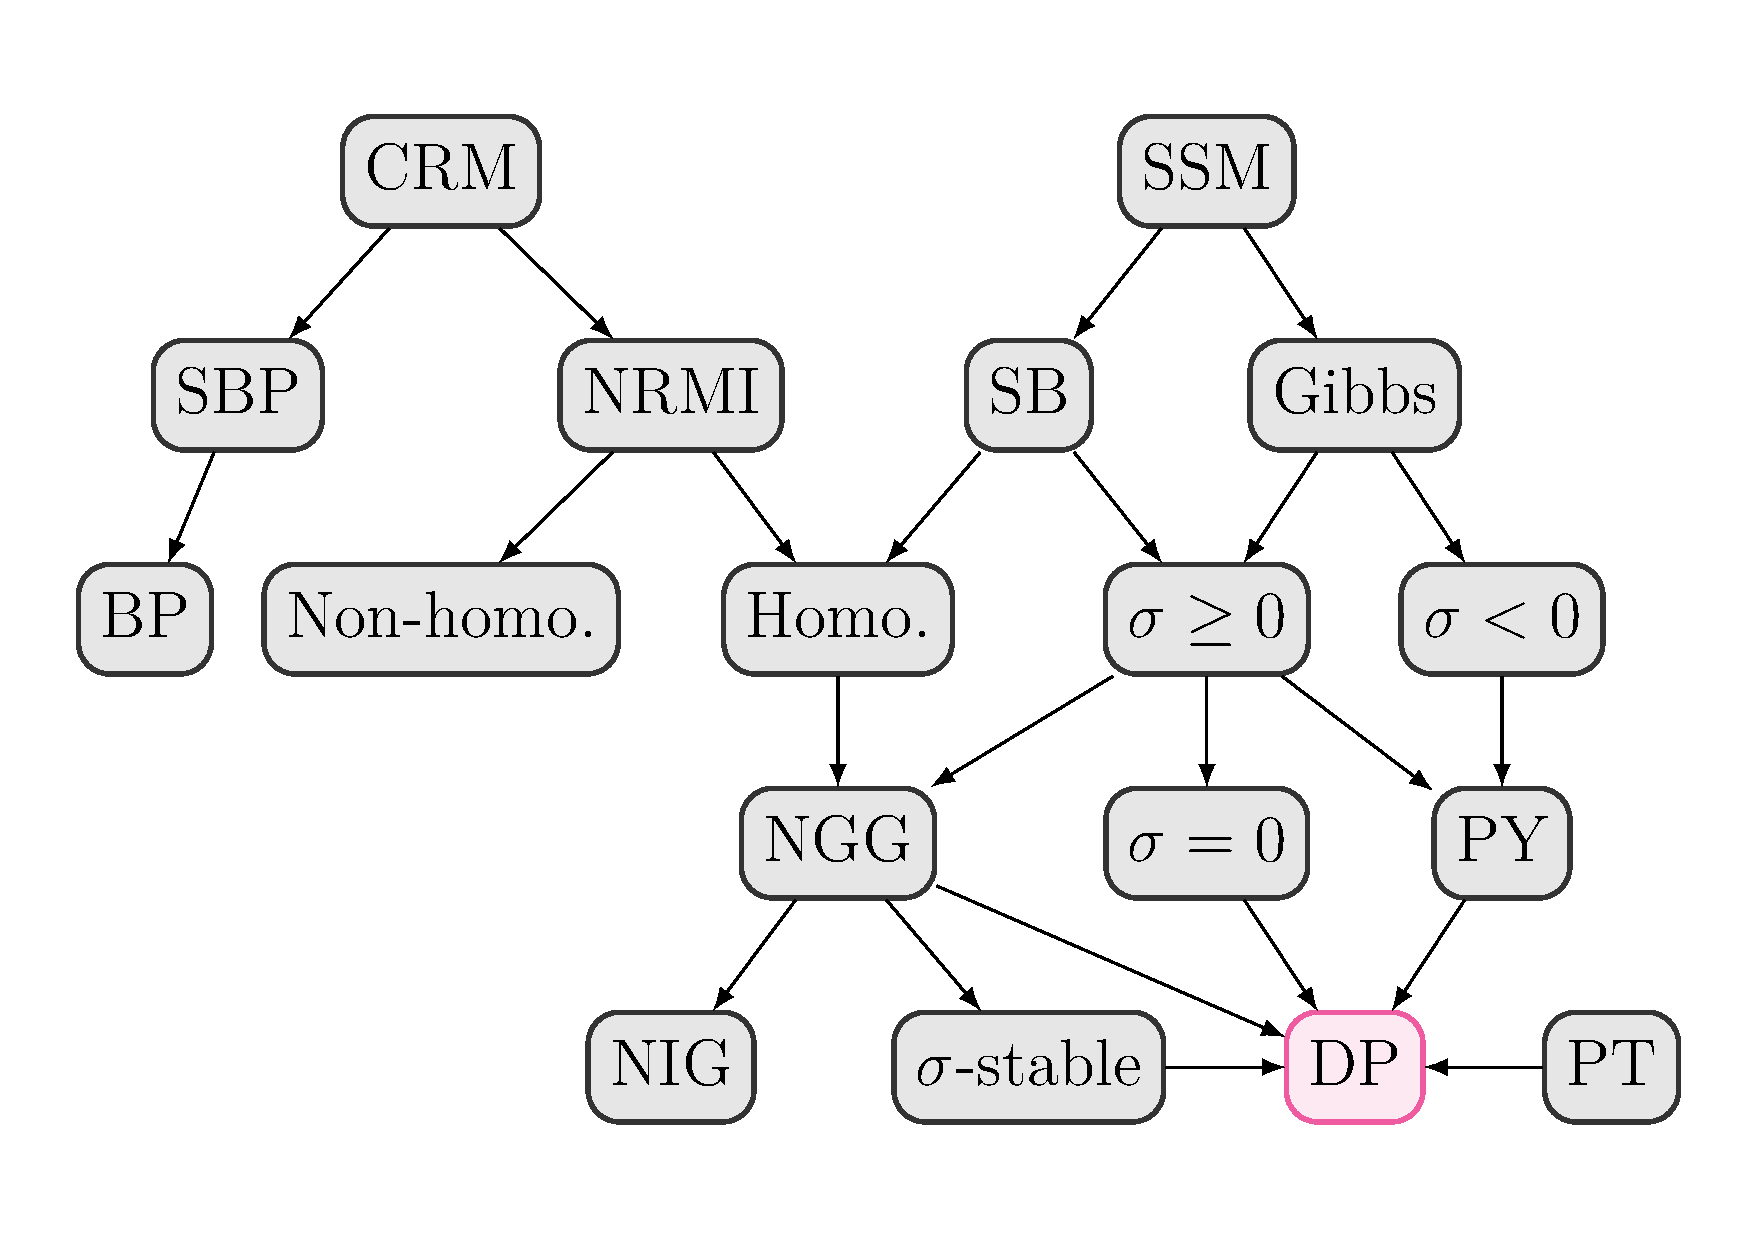
\includegraphics[width=\textwidth]{figures_julyan/introRPM/graph_model}}
\only<2>{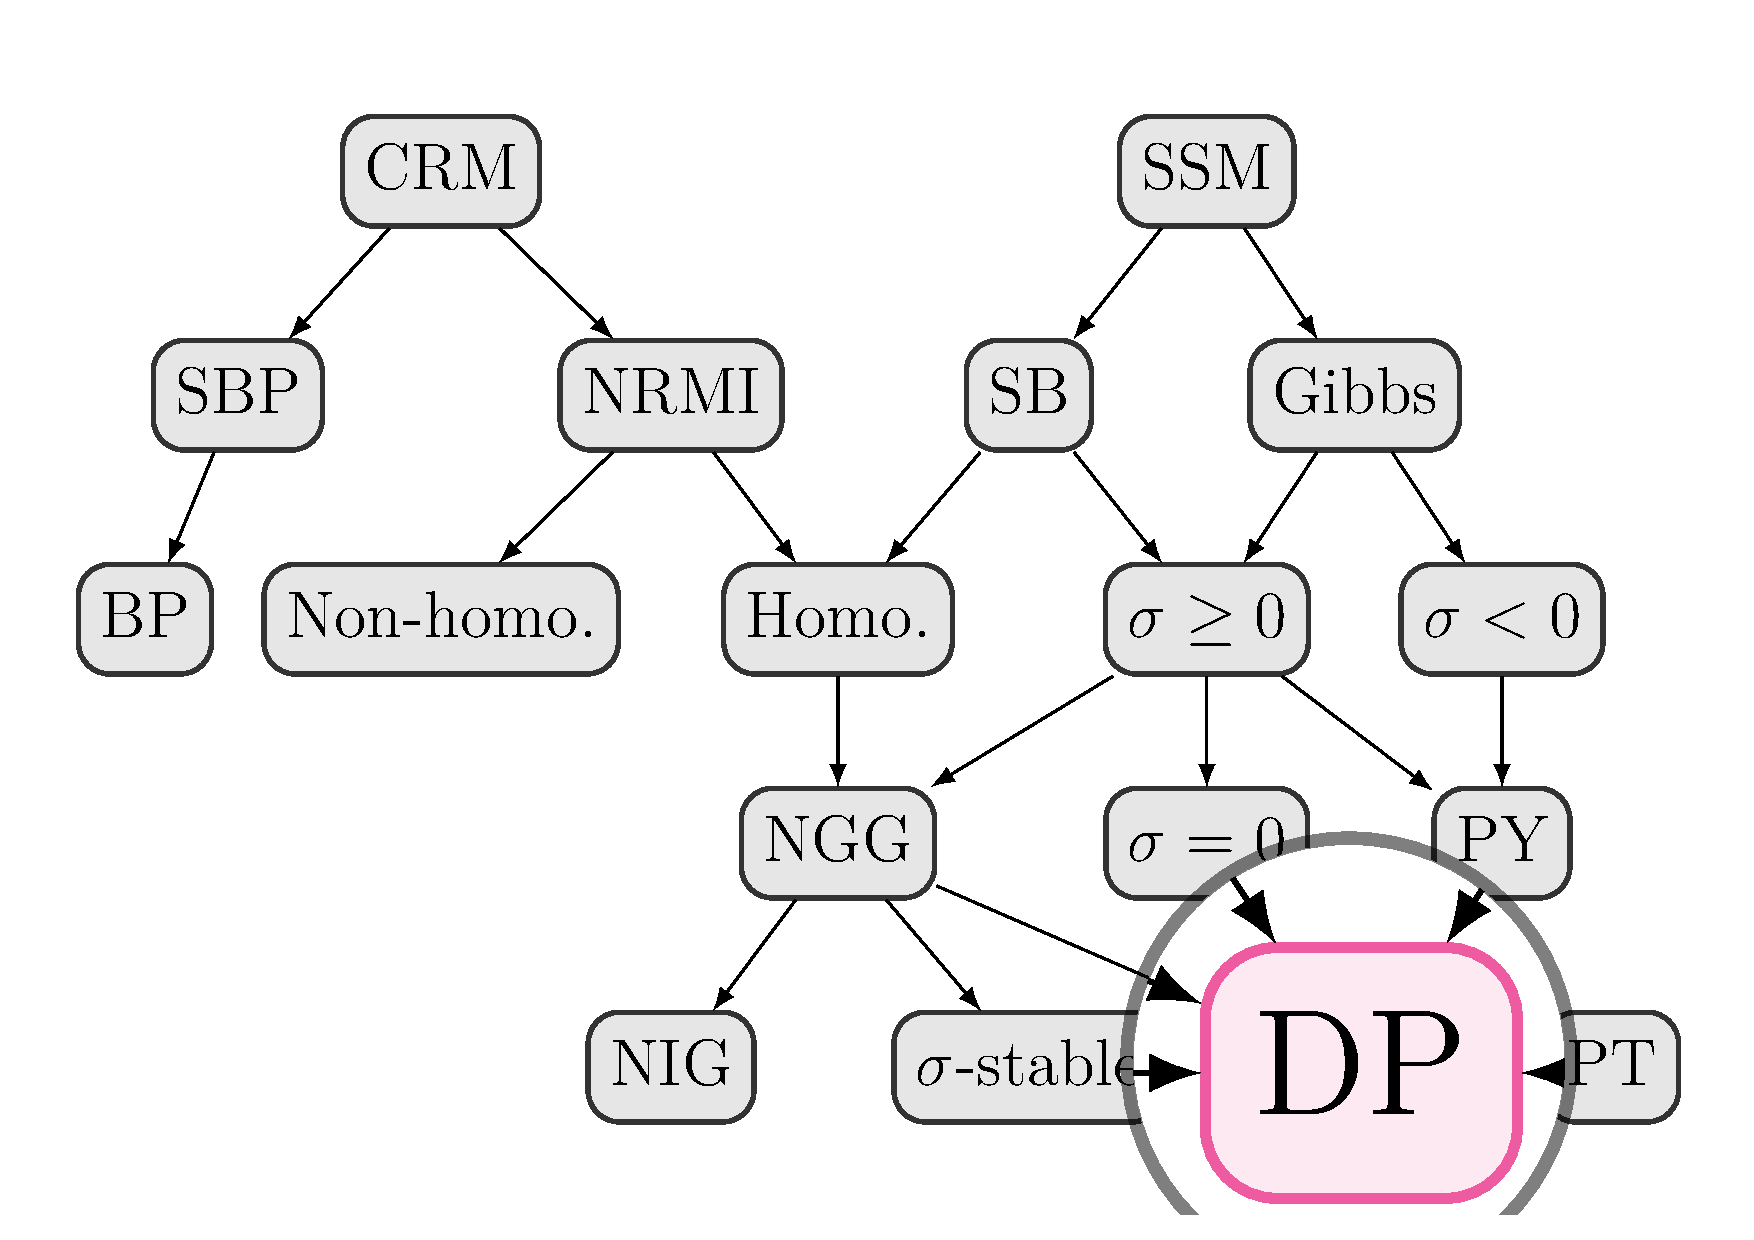
\includegraphics[width=\textwidth]{figures_julyan/introRPM/graph_model_dp}}
\end{frame}


%------------------
% PY

\begin{frame}[allowframebreaks]{Pitman--Yor process}
	\begin{proposition}
[Pitman Sampling formula] The multiplicities $(m_1,\ldots,m_n)$ in $X_1,\ldots, X_n|P\simiid P,\ P\sim PY(\sigma, \PrecisonParam P_0)$ have distribution
\begin{equation*}
    p(m_1,\ldots,m_n)=\frac{n!}{(1+\PrecisonParam)_{(n-1)}}(\PrecisonParam +\sigma)\cdots (\PrecisonParam+(k-1)\sigma)\prod_{\ell=1}^n\frac{1}{m_\ell!}\bigg(\frac{(1-\sigma)_{(\ell-1)} }{\ell!}\bigg)^{m_\ell}
\end{equation*}
\end{proposition}


\textbf{Proof.}
Same technique as for the DP ESF.



\framebreak

\begin{columns}

\column{.6\textwidth}
\begin{proposition}[Power law and $\sigma$-diversity]
For $\sigma >0$ we have the almost sure convergence 
$$
n^{-\sigma}K_n\rightarrow S_{\sigma, \PrecisonParam},
$$
where $ S_{\sigma, \PrecisonParam}$ is called $\sigma$-diversity of the PY, whose density is a polynomially tilted \alert{Mittag--Leffler density} (ML):
\begin{equation*}
    g_{\sigma,\PrecisonParam}(x)\propto x^{\PrecisonParam/\sigma}g_\PrecisonParam (x),
\end{equation*}
and $g_\alpha$ is ML density.
\end{proposition}
\column{.35\textwidth}
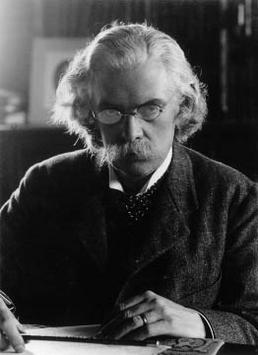
\includegraphics[width=\textwidth]{figures_julyan/trombi/Mittag-Leffler}
		\hfill\textcolor{gray}{[Image: Wikipedia]}
\end{columns}




\framebreak

\begin{theorem}[Stick breaking representation for PY]
If $V_j\simind Be(1-\sigma, \PrecisonParam + j\sigma)$ and $p_1=V_1,\ p_j=V_j\prod_{l<j}(1-V_l)$ and further we have $\phi_j\simiid P_0$ then 
$$
P=\sum_{j=1}^\infty p_j \delta_{\phi_j} \sim PY(\sigma,\PrecisonParam P_0).
$$
\end{theorem}

\framebreak


\begin{proposition}
[Moments of PY] If $P\sim PY(\sigma, \PrecisonParam P_0)$, then for every measurable sets $A,B$ we have
\begin{enumerate}
    \item[1)] $\E [P(A)] = P_0(A),$
    \item[2)] $\E[P(A)P(B)]=(1-\sigma)/(1+\PrecisonParam)P_0(A\cap B) + (\PrecisonParam + \sigma)/(1+ \PrecisonParam)P_0(A)P_0(B),$
    \item[3)] $\Cov[P(A),P(B)] = (1-\sigma)/(1+\PrecisonParam)\big(P_0(A\cap B) -P_0(A)P_0(B)\big)$.  
\end{enumerate}
\end{proposition}
\framebreak


\textbf{Proof.}
\begin{enumerate}
    \item[1)] We use the stick-breaking representation:
    \begin{equation*}
        \E P(A) =\sum_j \E p_j \E\delta_{\phi_j}=\sum_j \E(p_j) P_0(A) = P_0(A)\E (\sum_j p_j)= P_0(A).
    \end{equation*}
    \item[2)] Let $X_1, X_2|P \simiid P$, then
    \begin{equation*}
        \E(P(A)P(B)) = \P(X_1\in A, X_2\in B)=\P(X_1\in A)\P(X_2\in B|X_1\in A).
    \end{equation*}
    Lets investigate two terms above: from 1) we know that $\P(X_1\in A)=P_0(A)$. We know the predictive of PY:
    \begin{equation*}
        X_2|X_1 \sim \frac{\PrecisonParam + \sigma}{\PrecisonParam + 1}P_0+\frac{1-\sigma}{\PrecisonParam + 1}\delta_{X_1},
    \end{equation*}
    and hence
    \begin{equation*}
        \P(X_2\in B|X_1\in A) = \frac{\PrecisonParam + \sigma}{\PrecisonParam + 1}P_0(B) + \frac{1-\sigma}{\PrecisonParam + 1}P_{0A}(B),
    \end{equation*}
    when we used notation $P_{0A}(B)=P_0(B|A)=P_0(A\cap B)/P_0(A)$ for a conditional measure.
    \item[3)] It is straightforward combination of 1) and 2).
\end{enumerate}

\framebreak

Unlike the DP, PY is not conjugate under incoming independent samples. However, the posterior can be explicited.

\begin{theorem}
[Posterior distribution of PY] If $P\sim PY(\sigma, \PrecisonParam P_0)$ then the posterior of $P$ based on observations $X_{1:n}|P\simiid P$ has the distribution of the random probability measure
\begin{equation*}
    (1-q_n)P_n + q_n \sum_{j=1}^{K_n}p_j^*\delta_{X_j^*},
\end{equation*}
where $X^*_{1:n}$ are the $K_n$ distinct values in $X_{1:n}$, frequencies are referred to as $n_1,\ldots,n_{K_n}$ and 
\begin{itemize}
    \item $q_n\sim Beta(n-K_n \sigma, \PrecisonParam +K_n\sigma)$,
    \item $(p_1^*, \ldots, p^*_{K_n})\sim \Dir_{K_n}(n_1-\sigma, \ldots, n_{K_n} -\sigma)$,
    \item $P_n\sim PY(\sigma, (\PrecisonParam + \sigma K_n)P_0)$.
\end{itemize}
\end{theorem} 
\end{frame}

\begin{frame}{Impact of the stability parameter $\sigma$}
Prior distribution of the number of clusters $k_n$ 
\begin{itemize}
\item<1-> \textcolor<1>{red2}{$\alpha$ controls the location} (as for the DP)
\item<2-> \textcolor<2>{red2}{$\sigma$ controls the flatness (or variability)}
\end{itemize}
\visible<3->{
Example with $n=50, \alpha=1$ and \textcolor{red2}{$\sigma=0.2,0.3,\ldots, 0.8$}
}
\begin{center}
\visible<3->{\adjincludegraphics[width=.7\textwidth,trim={0 {.1\height} 0 {.12\height}},clip]{figures_julyan/introRPM/prior_K_n_PY.pdf}\\
	\hfill\textcolor{gray}{[Image by \citet{deblasi2015gibbs}]}
}
\end{center}
\end{frame}


\begin{frame}{Hierarchical Dirichlet process}
A nonparametric version of \textbf{Latent dirichlet allocation} \citep{blei2003latent} due to  \citet{teh2006hierarchical}\\
\begin{center}
		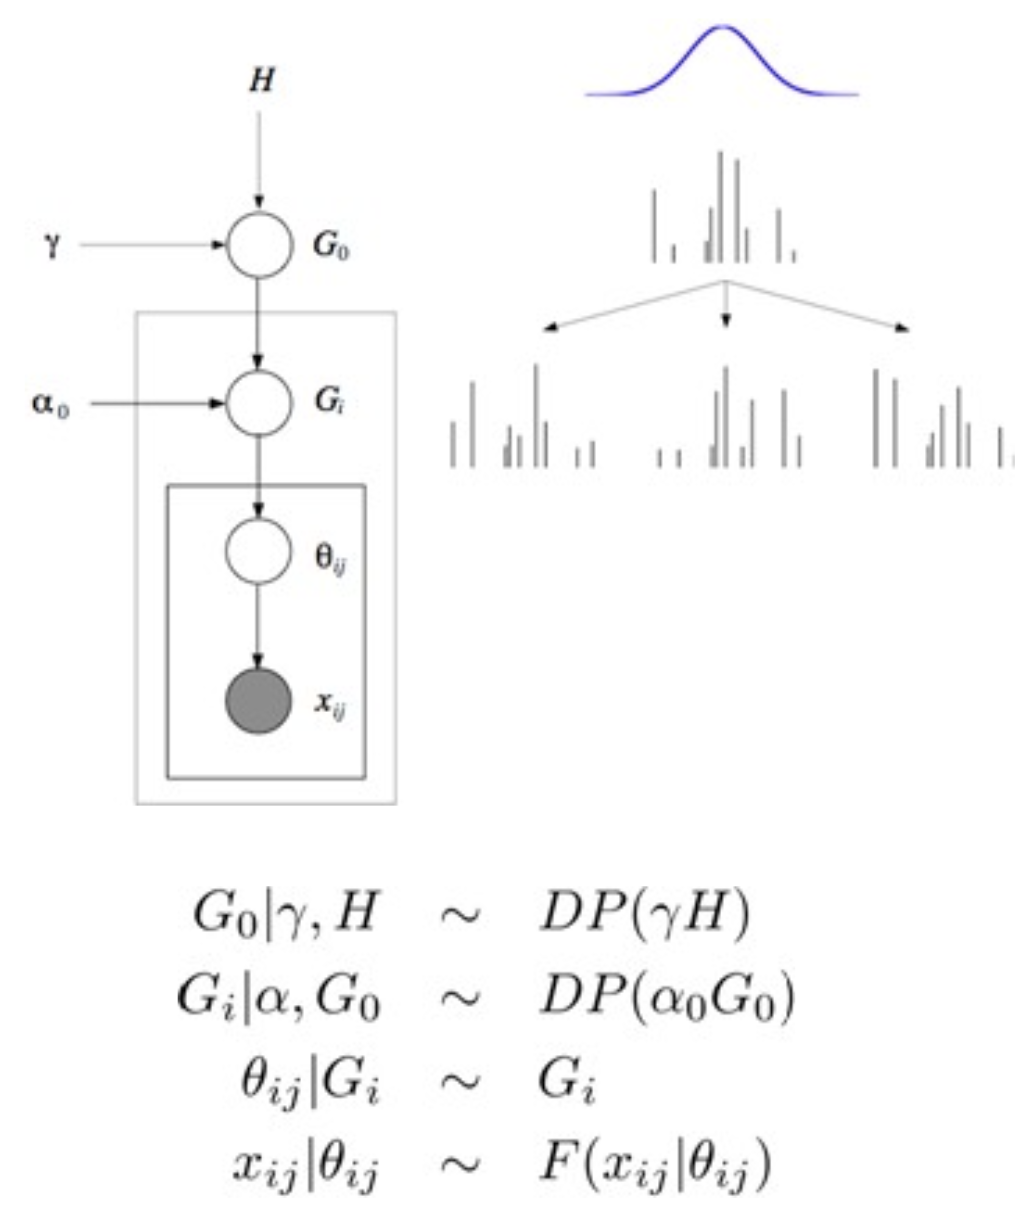
\includegraphics[width=.5\textwidth]{figures_julyan/beyond_DP/HDP}
\end{center}
\hfill\textcolor{gray}{[Image by M. Jordan]}
\pause
	
	Associated partition distr. called \alert{Chinese Restaurant Franchise}.
\end{frame}

\begin{frame}{Indian Buffet process}
	Feature allocation model by  \citet{ghahramani2006infinite}, where observations may share several features.\pause 	\alert{Generative model is as follows}
	\begin{itemize}[<+->]
		\item first customer samples $\text{Poisson}(\gamma)$ dishes
		\item second customer chooses every dish of first customer \textit{wp} $1/2$, plus  $\text{Poisson}(\gamma/2)$ new dishes
		\item $\ldots$
		\item $i$th step: $K$ dishes have been sampled, each by $n_1,\ldots,n_K$ customers;  $i$th customer chooses $j$th dish  \textit{wp} $n_j/i$, plus  $\text{Poisson}(\gamma/i)$ new dishes.
	\end{itemize}\pause
	
	\alert{Log growth}: $K_n\sim \text{Poisson}(\gamma\log n)$.
	
		\begin{center}
			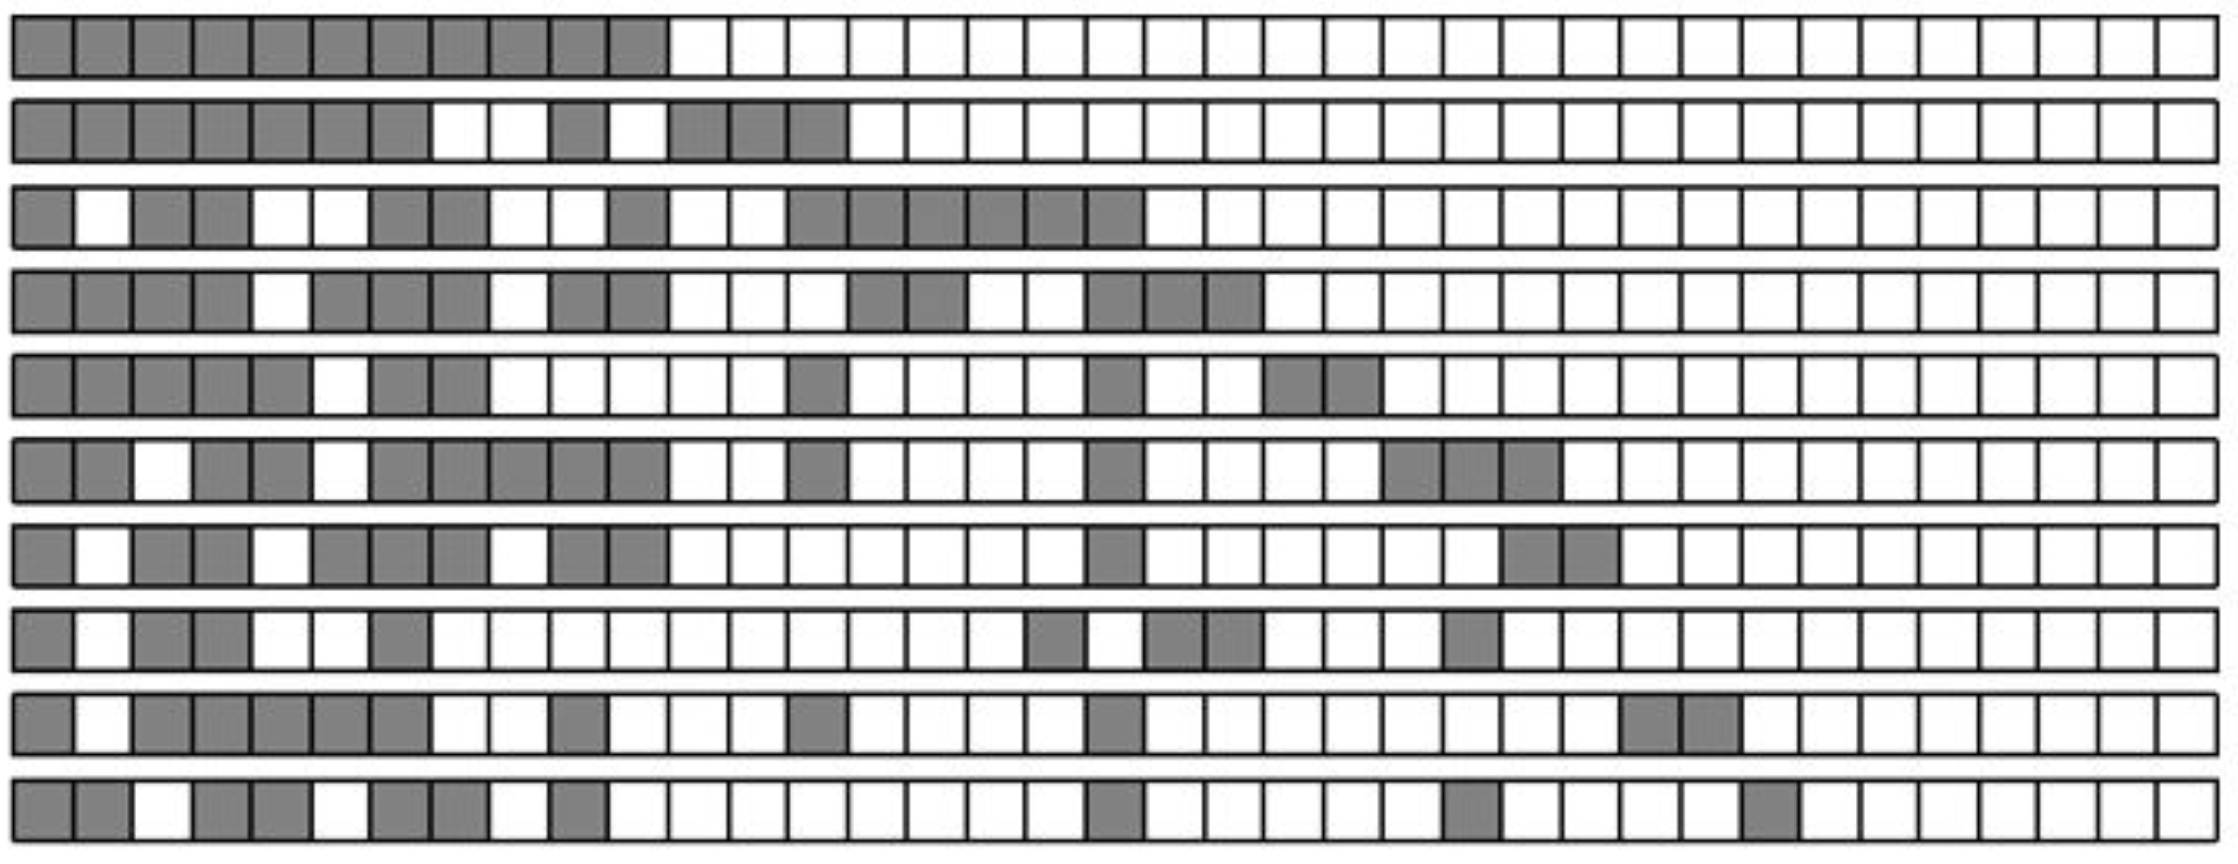
\includegraphics[width=.7\textwidth]{figures_julyan/beyond_DP/IBP_draw}
		\end{center}
		\hfill\textcolor{gray}{[Image by M. Jordan]}
\end{frame}

